%!TEX root = main.tex

\section{Solution Path}
\label{sec:solutionpath}
The proposed methodology gathers not only the knowledge about capabilities of high-thrust and low-thrust maneuvers, but also the features about the described mission and systems design, and the given cost model.
Several mission transfers are obtained and evaluated, and finally a Pareto Optimality yields the best multi-objective solutions.
The whole \emph{mission design} procedure is developed in Matlab framework.
\subsection{Strategy}
\label{subsec:strategy}
In the literature, to the best knowledge of the authors, emphasis is placed on characterizing a generic space transfer with solutions which maximize the final mass (or on-orbit mass, or net mass) for a fixed launch mass~\cite{Randolph:2002aa,Oleson:1997aa}.
In this work the aim is to enhance the efficiency of a GEO Hybrid Transfer when the payload's power and mass are specified (fixed), and the mission is analyzed through a \emph{top-down approach}. 
The aforementioned strategy characterizes the mission starting from the GEO and ends at LEO, in such a way that the mission characterization progresses ``backward'', or ``top-down'', as outlined in the following flowchart
%
\begin{center}
\smartdiagramset{
module minimum height = 0.6cm,%
module y sep = 1.4,%
back arrow disabled 
}
\smartdiagram[flow diagram:]{GEO,EP segment,CP segment,LEO}
\end{center}
%
On the one hand, every \emph{hybrid transfer} is payload-customized because the authors believe that the key feature in designing an EP is the payload power request, as outlined throughout the SA sizing.
On the other hand, the \emph{top-down} strategy produces complications to solve low-thrust and high-thrust transfers and to evaluate if the spacecraft mass at launch is feasible or not. 
For instance, the tables lookup \eqref{eq:fourtablelookup} and \eqref{eq:fivetablelookup} work for a fixed initial thrust-to-mass ratio $\tfrac{T}{m_0}$, while the backward strategy puts a mass constraint on a fraction of the delivered mass in GEO through \Eq{eq:masspayload}, the mass of trajectory-independent subsystem listed in \tablename\ref{tab:spacecraftbusforgeomission} and the $m_{sep}$ in \tablename\ref{tab:sepmassbudgets}.
\subsection{Flowchart}
\label{subsec:flowchart}
The whole flowchart is represented in \figurename\ref{fig:flowchart}, where the  implemented algorithm is shown step-by-step. In order to better understand this scheme, a clarification on how it is structured is required. Initially, the flow diagram can be examined through the \emph{coloring} of the blocks of which it is made up:
\begin{itemize}
\item \emph{Blue blocks} state the inputs of the \emph{Hybrid Transfers} simulation.
\item \emph{Green blocks} mark the tables lookup obtained offline.
\item \emph{Red blocks} are the ones that make choices along the algorithm-path.
\item \emph{Purple block} represents the \emph{Search Grid}. 
\item \emph{Orange blocks} contain data about  the technology the spacecraft is equipped with.
\item \emph{Black blocks} involve subsystems model, cost model and transfer performance evaluation. 
\end{itemize}
The flowchart can be red through the sequence of phase (on the right side of the analyzed figure) that compose the top-down strategy. 

The input values to start the analysis are the payload power, from which the payload mass is calculated \eqref{eq:masspayload}, and the life degradation factor of the SA ($L_d^{min}=\tfrac{P_{mp}}{P_{mp}}\big|^{min}_{\textsc{eol}}$) for the entire mission (transfer and the \textit{ } parking) and the lifetime in GEO ($LF_{geo}$), which is needed to compute the minimum coverglass required during the satellite’s on-orbit lifetime using equations \eqref{eq:xtjphi} and \eqref{eq:1yearphi}.
%
\begin{figure*}[htp]
\centering
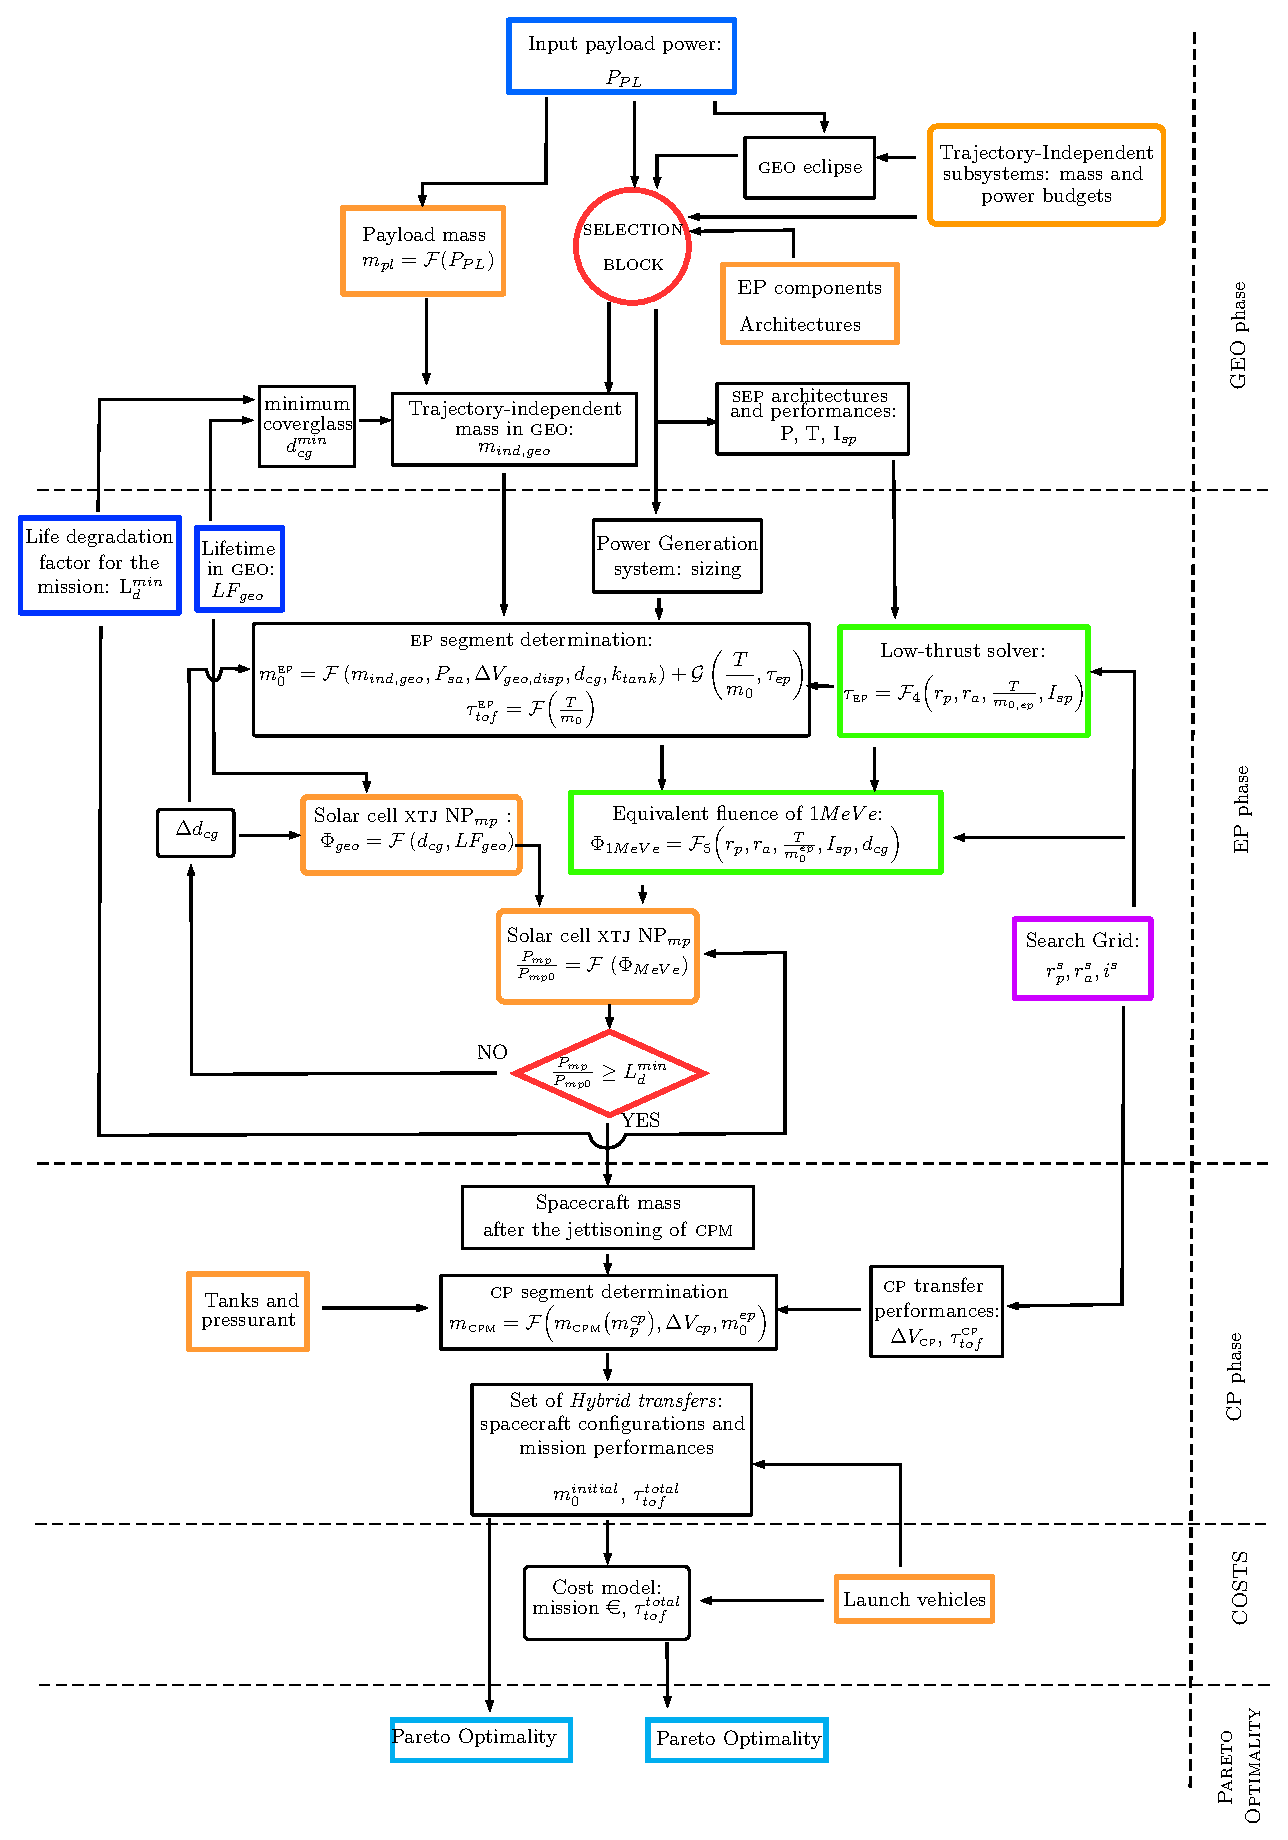
\includegraphics[width=0.8\textwidth]{blockdiagram_thesis.eps}
\caption{\textbf{Flowchart}}
\label{fig:flowchart}
\end{figure*}
%
The main blocks in \figurename\ref{fig:flowchart} from the top to the bottom are the following:
\begin{enumerate}
\item \emph{The Selection Block} (red circle) within the GEO phase. The algorithm chooses, among the six possibilities for the EP system (\tablename\ref{tab:electricpropulsionsystemmassbudgets}), the one that guarantees, through the power balance \eqref{eq:phat}, the maximum thrust \eqref{eq:thrustphat} along the EP segment. The resulting configuration is used whatever the HT, except for the FCT.
\item \emph{The EP segment determination} within the EP phase. The spacecraft mass before the low-thrust trajectory and EP time-of-flight are computed, with a guessed coverglass, by solving a nonlinear system.
\item \emph{The red diamond} at the bottom of the EP phase. If the $\Phi_{\scriptstyle{1~\si{\mega\electronvolt}}}^{\scriptstyle{mission}}$ leads to a power generation capability of the SA at the end-of-life greater than $L_d^{min}$, the procedure goes on. 
Otherwise, the coverglass is increased of $1\%$
\begin{equation}
d_{cg}\big|_{new} = (1+0.01)~d_{cg}\big|_{old}\label{eq.coverglassadd}
\end{equation}
and the evaluation of the low-thrust phase continues until $\tfrac{P_{\scriptstyle{mp}}}{P_{\scriptstyle{mp_{0}}}} \ge L{\scriptstyle{_d^{min}}}$.
This iterative method is necessary because if the coverglass mass changes, the EP transfer time and the initial mass of spacecraft will change consequently.
Then \emph{an iterative of each step is done starting from the evaluation of the initial mass of EP phase until the EOL power degradation requirement is met ($\tfrac{P_{\scriptstyle{mp}}}{P_{\scriptstyle{mp_{0}}}} \ge L{\scriptstyle{_d^{min}}}$ )}.
%
One might think that this is not an optimal design because the shielding mass will be oversized, thus the overall launch mass and cost will increase.

But if the increment value is wisely tuned, the burden mass
\begin{equation}
\Delta m = A{\scriptstyle_{sa}}\rho{\scriptstyle{_{cg}}}\Bigl(d_{cg}\big|_{new}\Bigr)~\Bigl(\dfrac{0.01}{0.01+1}\Bigr) \label{eq:burdenmasscoverglass}
\end{equation}
can be designed in such a way to estimate a threshold\footnote{$\rho_{cg} = 2550 ~\si{\kg\per\cubic\meter}$}.
Referring to the \figurename\ref{fig:burdencoverglassmass}, for instance, if the coverglass is thick $\sim 60~\si{\micro\meter}$ and the solar array area is ($\sim80~\si{\square\meter}$), the added mass is  $0.15~\si{\kilo\gram}$ at maximum.
%
\begin{figure}[htp]
\centering
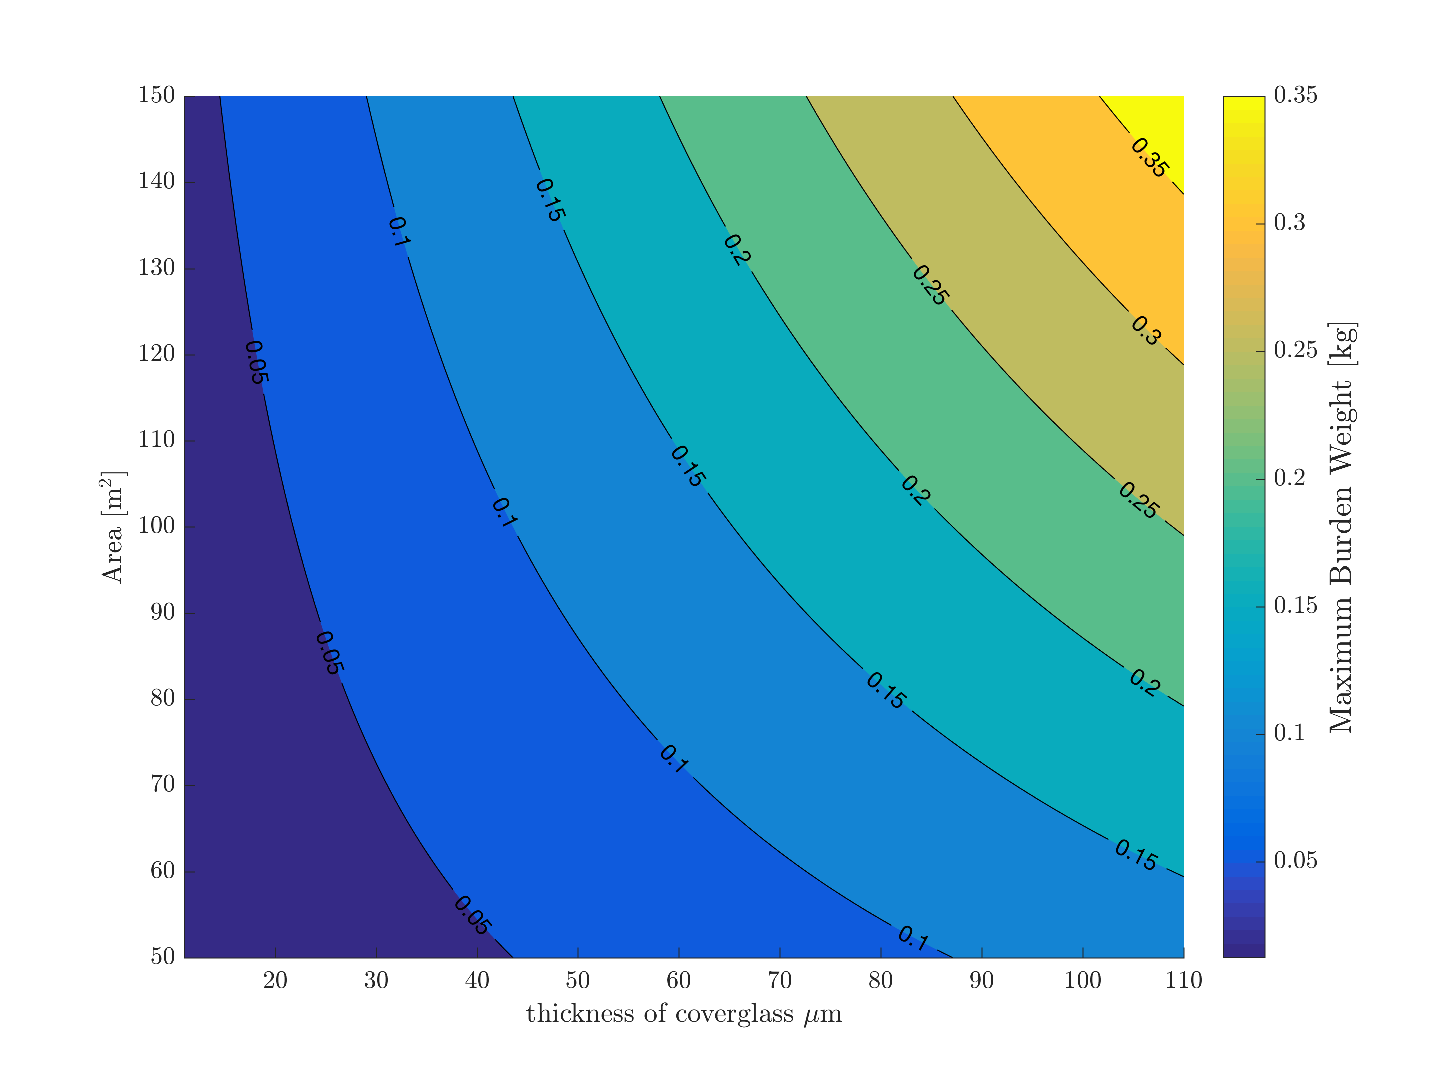
\includegraphics[width=0.5\textwidth]{deltamasscoverglass.eps}
\caption[Burden coverglass mass]{\textbf{Burden coverglass mass for} $\Delta d_{\scriptstyle{cg}} = 1.00\%$.}
\label{fig:burdencoverglassmass}
\end{figure}
\item \emph{The CP segment determination} for the CP phase analysis. The \textit{CPM} mass is computed; thus the spacecraft status in LEO is determined as well as the HT transfer, and the GEO mission is characterized.
\item \emph{Pareto optimality blocks} at the bottom of the flow diagram. Since the search grid block (purple rectangle) forces different trajectories, there will be a set of launched masses at LEO, transfer times to GEO and mission costs. 
Thus the \emph{best} solutions are picked by the Pareto criterion within two different framework: on the one hand there is the Pareto-efficient solutions for the mass-in-LEO vs. transfer time; on the other hand, Pareto-efficient transfers are refer to mission costs vs. transfer time.
\end{enumerate}